\chapter{Management process}
\section{Project start plan}
In deze sectie bespreken we de verwachte kost van het project. Voor de kostberekening maken we gebruik van het COCOMO I model. Als type project kiezen we tussen ``simple'', ``semidetached'' en ``embedded''. We kiezen hierin voor het type ``semidetached''. Dit weerspiegelt goed de huidige situatie van ons team. De omvang ons team is aan de grote kant en er zijn veel onbekende factoren in dit project (zie ook \ref{sec:risicoManagementPlan}). We gebruiken dan volgende formule:
\begin{equation*}
	E = a*KLOC^b
\end{equation*}
Hierbij is $E$ de ``effort'' uitgedrukt in persoonsmaanden (pm). Voor ons is het echter interessanter om naar de werkuren te kijken. Volgens de COCOMO standaard bevat \'{e}\'{e}n werkmaand 152 uren.  De benodigde tijd ($T$) kan dan als volgt berekend worden:
\begin{equation*}
	T = 152\frac{u}{pm}*E
\end{equation*}
Hierbij wordt T uitgedrukt in uren. Uit de tabellen van het COCOMO-model volgt dat $a = 3.0$ en $b = 1.12$. Verder schatten we in dat dit project een totale omvang zal hebben van 10KLOC. Dit geeft dan:
\begin{equation*}
	T = 152*3.0*10^{1.12} \approx 6011u 
\end{equation*}
Vermits ons team uit 7 personen bestaat, geeft dit per persoon een tijdsduur van:
\begin{equation*}
	T_{persoon} \approx 859u
\end{equation*}
Het spreekt voor zich dat dit duidelijk een overschatting is. $859u$ 
\section{Werk plan} \label{sec:workplan}
\subsection{Activiteiten}
Het project bestaat uit volgende activiteiten\footnote{In volgende versies van het SPMP komen hier nog verscheidene activiteiten bij.}, weergegeven als een work breakdown structure in figuur \ref{fig:workbreakdownstructure}.
\begin{figure} [H]
    \centering
    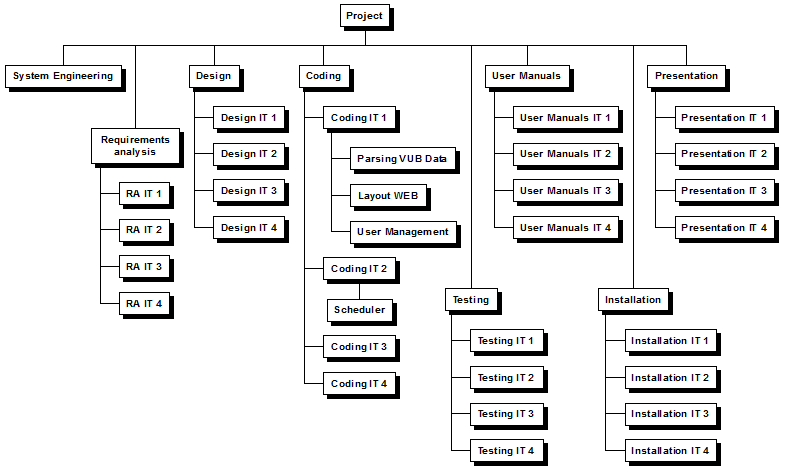
\includegraphics[width = \textwidth]{ManagerialProcess/WBSChart.png}
    \caption{Work breakdown structure.}
	\label{fig:workbreakdownstructure}
\end{figure}
Voor de eerste iteratie is de work breakdown structure weergegeven in figuur \ref{fig:wbsIteratie1}.
\begin{figure} [H]
	\centering
	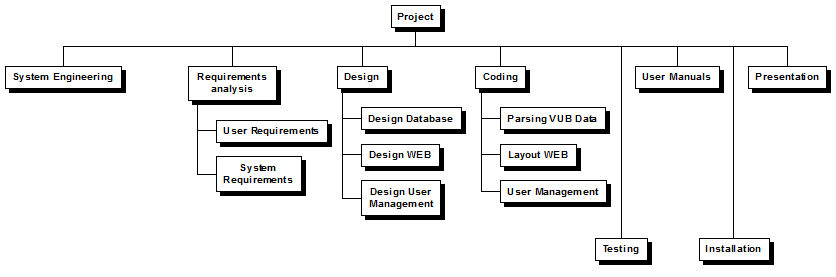
\includegraphics[width = \textwidth]{ManagerialProcess/WBSChartIteratie1.png}
	\caption{Work breakdown structure van iteratie 1.}
	\label{fig:wbsIteratie1}
\end{figure}
In de volgende versies van de SPMP zullen de work breakdown structures van de volgende iteraties worden weergegeven.
\subsection{Planning}
In tabel \ref{tab:ActivityDependenciesIteratie1} is een overzicht weergegeven van de verschillende activiteiten gedurende iteratie 1. Hierbij zijn ook de afhankelijkheden weergegeven tussen deze activiteiten. Op basis van deze tabel kunnen we een Gantt chart opstellen en het kritisch pad bepalen.
\begin{table} [H]
	\centering
	\caption{Activiteiten van de eerste iteratie en afhankelijkheden.}
	\begin{tabular} {c|l|c|c}
		Activiteit ID & Activiteit Naam & Tijdsduur (in dagen) & Afhankelijkheden \\
		\hline
		1 & System Engineering & 21 & \\
		2 & Requirements Analysis & 14 & \\
		2.1 & User Requirements & 7 & \\
		2.2 & System Requirements & 7 & 2.1 \\
		3 & Design & 14 & 2 \\
		3.1 & Design Database & 5 & \\
		3.2 & Design WEB & 4 & \\
		3.3 & Design User Management & 5 & \\
		4 & Coding & 14 & \\
		4.1 & Coding Parsing VUB Data & 7 & 3.1, Release data dump \\
		4.2 & Coding Layout WEB & 14 & 3.2 \\
		4.3 & Coding User Management & 14 & 3.3 \\
		5 & Testing & 7 & 4 \\
		6 & User manuals & 3 & 4 \\
		7 & Installation & 1 & 5,6 \\
		8 & Presentation & 3 & 7	
	\end{tabular}
	\label{tab:ActivityDependenciesIteratie1}
\end{table}
Op basis van tabel \ref{tab:ActivityDependenciesIteratie1} bekomen we de Gantt chart voor iteratie 1 weergegeven in figuur \ref{fig:GantChartIT1}. Het kritisch pad is weergegeven in het rood. Hierbij is nog rekening met extra constraints:
\begin{itemize}
	\item Het project is gestart op 7 oktober 2013.
	\item De activiteit ``Requirements Analysis'' kan niet vroeger beginnen dan 21 oktober 2013.
	\item De activiteit ``Parsing VUB Data'' kan niet vroeger beginnen dan 18 november 2013 (zie tabel \ref{tab:kalender}).
	\item De activiteit ``Installation'' mag niet later eindigen dan 13 december 2013 (zie tabel \ref{tab:kalender}).
	\item De activiteit ``Presentation'' mag niet later eindigen dan 18 december 2013 (zie tabel \ref{tab:kalender}).
\end{itemize}
\begin{figure} [H]
	\centering
	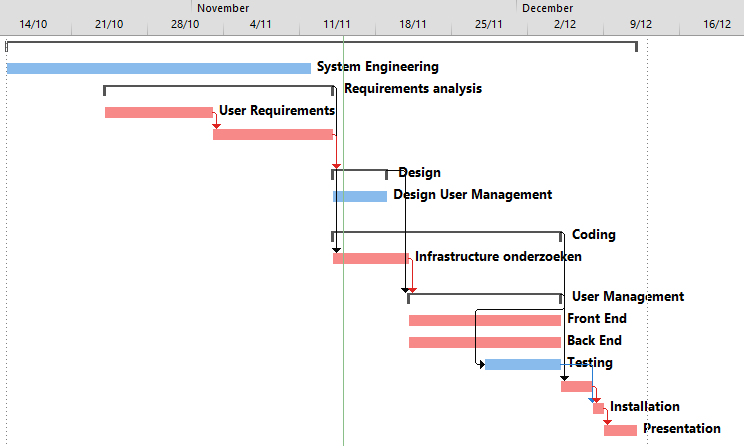
\includegraphics[width = \textwidth]{ManagerialProcess/GanttChartIT1.png}	
	\caption{Gantt chart voor iteratie 1.}
	\label{fig:GantChartIT1}
\end{figure}
Het kritisch pad begint bij de activiteit ```Parsing VUB Data''.  Vermits de datadump van de VUB pas ter onze beschikking wordt gesteld op 18 november, kunnen we hier niet vroeger aan beginnen.
%\subsection{Middelen}
%This subclause of the SPMP shall provide a detailed itemization of the resources allocated to each major work activity in the project work breakdown structure. Resources shall include the numbers and required skill levels of personnel for each work activity. Resource allocation may include, as appropriate, personnel by skill level and factors such as computing resources, software tools, special testing and simulation facilities, and administrative support. A separate line item should be provided for each type of resource for each work activity. A summary of resource requirements for the various work activities should be collected from the work packages of the work breakdown structure and presented in tabular form.
%Voor de design-activiteiten zal er gebruik worden gemaakt van een UML Designer \footnote{De specifieke tool die we gaan gebruiken is nog onder overleg.}. Het coderen zal gebeuren in Eclipse. 

\section{Controle plan}
\subsection{Requirements controle} \label{RequirementsControlPlan}
Op de website van het team \cite{portalWebsite} zal er een pagina beschikbaar zijn die het mogelijk maakt om zaken te rapporteren, en veranderingen te controleren met betrekkeing tot de SRS.
\\
\\
Er zal een requirements dashboard beschikbaar zijn die een overzicht weergeeft van alle requirements en hun status per iteratie (done, busy, planned, deferred, ... ). Hierbij worden telkens de belangrijkste statistieken per requirement weergegeven (percentage afgewerkt indien bezig, duurtijd implementatie indien klaar, aantal unit tests, ... ).

\subsection{Planning controle}
Voor het opvolgen en schatten van de planning zal ook gebruik worden gemaakt van de website \cite{portalWebsite}. Door gebruik te maken van een eigen implementatie beschikken we over voldoende flexibiliteit. Bovendien is bijvoorbeeld het gebruik van Microsoft Project \cite{MicrosoftProject} niet bevorderend voor het gebruik in teamverband. Door alles gecentraliseerd op de website te plaatsen kan elk teamlid gemakelijk aan de meest recente project gegevens.

\subsection{Budget controle}
Op de website van het team \cite{portalWebsite} zal er gebruik gemaakt worden van een time tracking tool die het mogelijk maakt een gedetailleerd logboek bij te houden van de reeds uitgevoerde activiteiten. Op basis hiervan kunnen we dan de ``kost'' berekenen van het project. 
\\
\\
De tijdsregistratie wordt uitgevoerd bij het be\"{e}ndigen van elke werkdag. Hierbij wordt telkens opgegeven aan welke activiteit men gewerkt heeft (een overzicht van de verschillende activiteiten bevindt zich in sectie \ref{sec:workplan}).

\subsection{Kwaliteitscontrole}
Ook de kwaliteit zal opgevolgd worden met behulp van de website. De quality assurance leader zal verantwoordelijk zijn voor de kwaliteitspagina op de website.

\subsection{Rapportering} \label{sec:rapportering}
In tabel \ref{tab:kalender} worden de deliverables voor dit project weergegeven. Hierrond worden volgende afspraken gemaakt:
\begin{itemize}
\item Alle documenten en source code (inclusief unit tests) worden per mail aangeleverd als een enkele zipfile, met als naam se2-iterM, waarbij M het nummer van de iteratie is (voor eerste versie van documenten geldt M = 0). De aanlevering gebeurt ten laatste voor 9u00 ’s ochtends op de dag van de deadline (zie tabel \ref{tab:kalender}).
\item Alle documenten en source code worden worden overeenkomstig getagd/gebranchd (se2-iterM) in de GitHub repository.
\item Andere artefacten (zoals executables) worden apart aangeleverd (direct, of via een link, in de opleveringsmail) en vermelden duidelijk de overeenkomstige iteratie in de bestandsnaam.
\item De mail van de oplevering bevat een bondig overzicht (lijstje) van wat er precies opgeleverd
wordt.
\end{itemize}
Voor het verspreiden van de resultaten zal ook gebruik worden gemaakt van de website. 
\begin{itemize}
\item Opgeleverde documenten, source code en andere artefacten moeten publiekelijk en overzichtelijk beschikbaar zijn.
\item Het opleveren van documenten en code per iteratie houdt in dat ten laatste op die welbepaalde dag (zie tabel \ref{tab:kalender}) de site ook up-to-date wordt gebracht.
\end{itemize}
Een presentatie duurt een half uur per groep en wordt ingevuld door 2 sprekers. Alle groepsleden moeten minimum \'{e}\'{e}n keer presenteren. De volgende zaken worden besproken of gedemonstreerd:
\begin{itemize}
\item een demo van de toegevoegde functionaliteit ten opzichte van de vorige iteratie
\item analyse van de ontmoete obstakels en de genomen beslissingen
\item bespreking van de functionaliteiten die aan bod zullen komen in de volgende iteratie
\item bespreking van eventuele obstakels, risico’s, etc. in de volgende iteratie
\item overzicht van de architectuur en design van de applicatie
\item bespreking van de statistieken zoals de tijd per taak en per persoon en van de eventuele vertragingen (plus oplossingen om deze zo klein mogelijk te houden en te vermijden in de toekomst)
\end{itemize}

\subsection{Metriek verzamelingsplan}
Metrieken zullen verzameld worden met behulp van de Eclipse Metrics Plugin \cite{EclipseMetricsPlugin}. Verzamelde metrieken zullen op de webpagina van het team gevisualiseerd worden.
\\
\\
Er zullen metrieken op methodenniveau en klassenniveau verzameld worden. Op methodenniveau verzamelen we volgende metrieken:
\begin{enumerate}
	\item 
		Cyclomatic Complexity.
		\\
		\\ %TODO Nakijken.
		Deze metriek geeft een indicatie van het aantal `lineaire' segementen in een methode (m.a.w. stukken code met geen branches). Dit kunnen we onder andere gebruiken om het aantal tests te bepalen om volledige dekking te krijgen. Het geeft ook een indicatie van de complexiteit van de methode.
		
	\item 
		Aantal statements
		\\
		\\
		Om de grootte van de methode te onderhouden, maken we gebruik van het aantal statements binnen een methode. Deze metriek is robuuster dan het aantal lijnen code vermits deze onafhankelijk is van de gebruikte programmeerstijl.
	\item
		Aantal levels.
		\\
		\\
		Deze metriek geeft het maximaal aantal geneste lagen in een methode. Een hoog aantal levels geeft aan dat we te maken hebben met een complexe  methode. Deze methoden kunnen vereenvoudigd worden door het extraheren van verscheidene private methoden.
	
	\item
		Aantal lokale variabelen in de scope.
		\\
		\\
		Deze metriek geeft het maximaal aantal lokale variable dat zich in de scope bevindt gedurende elk mogelijk punt in de methode. Een groot aantal wijst op complexe methoden.
	\item
		Aantal parameters.
		\\
		\\
		Deze metriek bevat het aantal parameters dat doorgegeven wordt aan een methode. Een te hoog aantal parameters wijst erop dat er te weinig gebruik gemaakt wordt van klassen.
	
	%TODO Feature Envy: vrij complex maar kan handig zijn

\end{enumerate}
Op klassenniveau verzamelen we volgende metrieken:
\begin{enumerate}
	\item 
		Efferent Couplings.
		\\
		\\
		In deze metriek wordt er gemeten hoeveel andere klassen de huidige klasse kent. Een hoog aantal koppelingen is nadelig voor de betrouwbaarheid van de code vermits het afhankelijk is van verscheidene types. Door de klasse op te delen in verscheidene deelklassen, kunnen we het aantal koppelingen naar omlaag brengen.
	\item
		Aantal velden.
		\\
		\\ %TODO wat zijn velden ?
		Deze metriek meet het aantal velden in een klasse. Bij een groot aantal velden moet er nagegaan worden of er verscheidene velden kunnen gegroepeerd worden in deelklassen.
	
	\item
		Complexiteit
		\\
		\\
		Deze metriek wordt berekend door de som te nemen van de Cyclomatic Complexities van de verschillende methoden die zich in deze klasse bevinden. Deze stelt dus de complexiteit voor van de gehele klasse.
		
	\item 
	{
		Cohesie tussen de verschillende methodes.
		\\
		\\
		De cohesie tussen de verschillende methoden in \'{e}\'{e}n enkele klasse is een belangrijk concept bij object georienteerd programmeren. De cohesie geeft aan of de klasse \'{e}\'{e}n of meerdere abstracties voorstelt. Indien \'{e}\'{e}n klasse meerdere abstracties voorstelt, moet deze opggesplitst worden in meerdere klassen waarbij elke klassen \'{e}\'{e}n abstractie voorstelt.
		\\
		\\
		Wij zullen de Henderson-Sellers metriek gebruiken \cite{HendersonSellers}. Om deze te berekenen voeren we volgende variabelen in: 
		$$ M = \{ m | \text{m is methode van de klasse} \} $$
		$$ F = \{ f | \text{f is een veld van de klasse} \} $$
		$$ r : F \rightarrow \mathbb{N} $$
Hierbij berekent $r(f)$ het aantal methoden dat veld $f$ aanroept. Vervolgens defini\"{e}ren we ook $\bar{r}$ als het gemiddelde van $r(f)$ over $F$. De Henderson-Seller metriek wordt dan berekent als:
		$$ HS = \frac{\bar{r} - |M|}{1 - |M|} $$
		Hoe lager de waarde, hoe beter de cohese tussen de verschillende methoden.
	} %TODO eventueel referentiewaarde en verklaren vanuit formule
\end{enumerate}

\section{Risico management plan} \label{sec:risicoManagementPlan}
In deze paragraaf zullen de verschillende risico's verbonden aan dit project besproken worden. In paragraaf \ref{sec:riskPriority} zullen deze risico's gepriotiseerd worden. Om de risico's te kunnen prioritiseren zullen we gebruiken maken van 3 parameters:
\begin{itemize}
	\item 
		De kans $p$ waarmee dit risico kan voorkomen. Hierbij is $ p \in \{1, 2, \ldots , 10\} $. Verder betekent $p = 1$ dat het risico niet kan voorkomen en $p = 10$ dat het risico met zekerheid voorkomt.
	\item 
		De impact $i$ op het project wanneer het risico werkelijkheid wordt. Hierbij is $ i \in \{1, 2, \ldots , 10\} $. Verder betekent $i = 1$ een impact op het project die minimaal is en $i = 10$ een impact die maximaal is.
	\item 
		De kost $c$ die het risico heeft op het project om het probleem op te lossen. Hierbij is $ c \in \{1, 2, \ldots , 10\} $. Hierbij betekent $c = 1$ een lage kostprijs, terwijl $c=10$ een hoge kostprijs betekent. Bij een hoge kostprijs zal de prioriteit van het risico lager gesteld worden, vermits het dan beter kan zijn om pas het risico weg te werken wanneer het voorkomt. Hiermee worden grote onnodige kosten vermeden.
		
\end{itemize}
\subsection{Project risico's}
\subsubsection{Niet-realistische Planning}
%TODO link leggen met geschatte budget: zie COCOMO I & II -> waren niet realistisch
Om de vooropgestelde deadlines (zie tabel \ref{tab:kalender}) te bereiken dient men voldoende tijd vrij te maken. Het zwaartepunt van het academiejaar van de verschillende groepsleden ligt bij de meeste groepsleden in het eerste semester. Het grootste risico in verband met planning ligt dus vooral bij de eerste iteratie. Dit kan het best vermeden worden door gebruik te maken van interne deadlines en de progressie op te volgen tijdens de wekelijkske teammeetings.
\\
\\
We karakteriseren dit risico m.b.v. volgende parameters:
\begin{align*}
	p &= 8\\
	i &= 8\\
	c &= 2
\end{align*}

\subsection{Technische risico's}
\subsubsection{Gebrek aan ervaring in de implementatie-technologie}
Hiervoor wordt er gekeken naar de programmeertalen die gebruikt worden tijdens dit project (zie sectie \ref{sec:languages}). Een overzicht van de aanwezige kwaliteiten is zichtbaar in tabel \ref{tab:skilllevel}. Wat opvalt is dat er van elks kwaliteiten aanwezig zijn, maar er zijn ook de nodige aandachtspunten. Zo is bijvoorbeeld de ervaring in Java en JavaScript beperkt.

\begin{table} [htbp]
	\centering
  	\caption{Ervaring van de verschillende teamleden.}
    \begin{tabular}{c|ccccl}
  		  	& Java 	& JavaScript & HTML \textbackslash CSS 		& SQL 	& Opmerkingen \\
  		  	\hline
  		  	Christophe & -	& ++ 		& ++ 		& ++ & \shortstack{ Reeds ervaring opgedaan \\ in de bedrijfswereld} \\
  		  	Youri & + & - & - & ++ & \shortstack{Voorkeur voor logica, \\ A.I. en modeleren.} \\
  		  	Nicolas & + & - & + & ++ & Voorkeur voor back end \\
  		  	Tim & - & - & + & ++ & \shortstack{Reeds ervaring in C++ en \\ andere programmeerprojecten} \\
  		  	Sam & + & - & + & ++ & \\
  		  	Fernando & - & - & + & ++ & Voorkeur voor design \\
  		  	Pieter & ++ & + & + & + & \shortstack{Reeds ervaring opgedaan \\ in de bedrijfswereld}
    \end{tabular}
  	\label{tab:skilllevel}
\end{table}
Omdat de implementatie-technologie opgelegd wordt, is het gebruik maken van andere frameworks, programmeertalen, ... geen optie. Hierdoor zullen we gebruik maken van workshops. Hiermee gaan we de ervaringen van de verschillende teamleden op elkaar overbrengen. Een workshop wordt georganiseerd door een teamlid die zijn kennis en ervaringen over een bepaalt framework, programmeertaal, ... uiteenzet gedurende 30 \`{a} 60 minuten. Volgende workshops zijn reeds gepland:
\begin{itemize}
	\item GitHub (door Christophe)
	\item Java (door Pieter)
\end{itemize}
Doordat we gebruik maken van korte workshops, zou de invloed van deze workshops op de planning minimaal zijn. We karakteriseren dit risico m.b.v. volgende parameters:
\begin{align*}
	p &= 8\\
	i &= 8\\
	c &= 4
\end{align*}

\subsubsection{Gebrekkige performantie}
Het hoofddoel van dit project is het maken van een scheduler. Het is uiteraard gewenst dat het schedulen vlot verloopt. Vanwege de complexiteit van dit onderwerp zal er ook de nodige aandacht besteedt moeten worden aan de performantie van de scheduler.
\\
\\
Dit zal gemonitored worden met behulp van benchmarks. Indien er tekortkomingen ontdekt worden, zullen de nodige optimalisaties moeten doorgevoerd worden aan de scheduler. We karakteriseren dit risico m.b.v. volgende parameters:
\begin{align*}
	p &= 7\\
	i &= 2\\
	c &= 7
\end{align*}


\subsection{Bedrijfsrisico's}
\subsubsection{Ontwikkelen van de verkeerde functionaliteit}
Het ontwikkelen van verkeerde functionaliteit is steeds een re\"{e}el risico. Doordat we gebruik maken van een iteratief development process, waarbij we bij elke iteratie werkende code opleveren, krijgen we geregeld feedback van de klant. Hierdoor kunnen we de requirements, indien nodig, bijsturen. Vermits we bij de start van elke iteratie een gedetailleerde planning opstellen, kunnen eventuele wijzigingen vlot verwerkt worden. We karakteriseren dit risico m.b.v. volgende parameters:
\begin{align*}
	p &= 6\\
	i &= 7\\
	c &= 4
\end{align*}

\subsection{Prioriteit van de verschillende risico's.} \label{sec:riskPriority}
Op basis van de 3 parameters $p$, $i$ en $c$ berekenen we de prioriteit $P$ van het risico. %TODO referentie naar boek software engineering %TODO tabel invullen
$$ P = (11 - p)*(11 - i)*c$$
Vermits hoge waarden van $p$, $i$ en $c$ belangrijker zijn, zijn de risico's met de kleinste waarden van $P$ het belangrijkste. Een (gesorteerd) overzicht is weergegeven in tabel \ref{tab:riskPriorityTabel}.
\begin{table} [H]
	\centering
	\caption{}
	\begin{tabular} {l|ccc|c}
		Risico & $p$ & $i$ & $c$ & $P$ \\
		\hline
		Niet-realistische planning 	& 8 	& 8 	& 2 	& 18 \\
		Gebrek aan ervaring 		& 8 	& 8 	& 4 	& 36 \\
		Verkeerde functionaliteit 	& 6 	& 7 	& 4 	& 80 \\
		Performantie 				& 7 	& 2 	& 7 	& 252\\

	\end{tabular}
	\label{tab:riskPriorityTabel}
\end{table}

%\section{Project closeout plan} niet.